\section{Additional Experiments}
\label{app:additional_exp}

This appendix provides additional experimental results to supplement the findings presented in the main paper. We offer a more granular breakdown of the 300B token experiment, analyze performance at a smaller 50B token scale to assess the generalization of our results, and report the results of a model red-teaming analysis to evaluate the model's safety profile.

\subsection{300B Experiment - Detailed Results}
\label{app:additional_exp_tasks_300B}

The detailed results for each evaluated task (contributing to the average over 10 tasks as shown in Figure \ref{fig:300b_performance} ) are given in Figure~\ref{fig:per_dataset_performance}.

\begin{figure}[ht] 
    \centering
    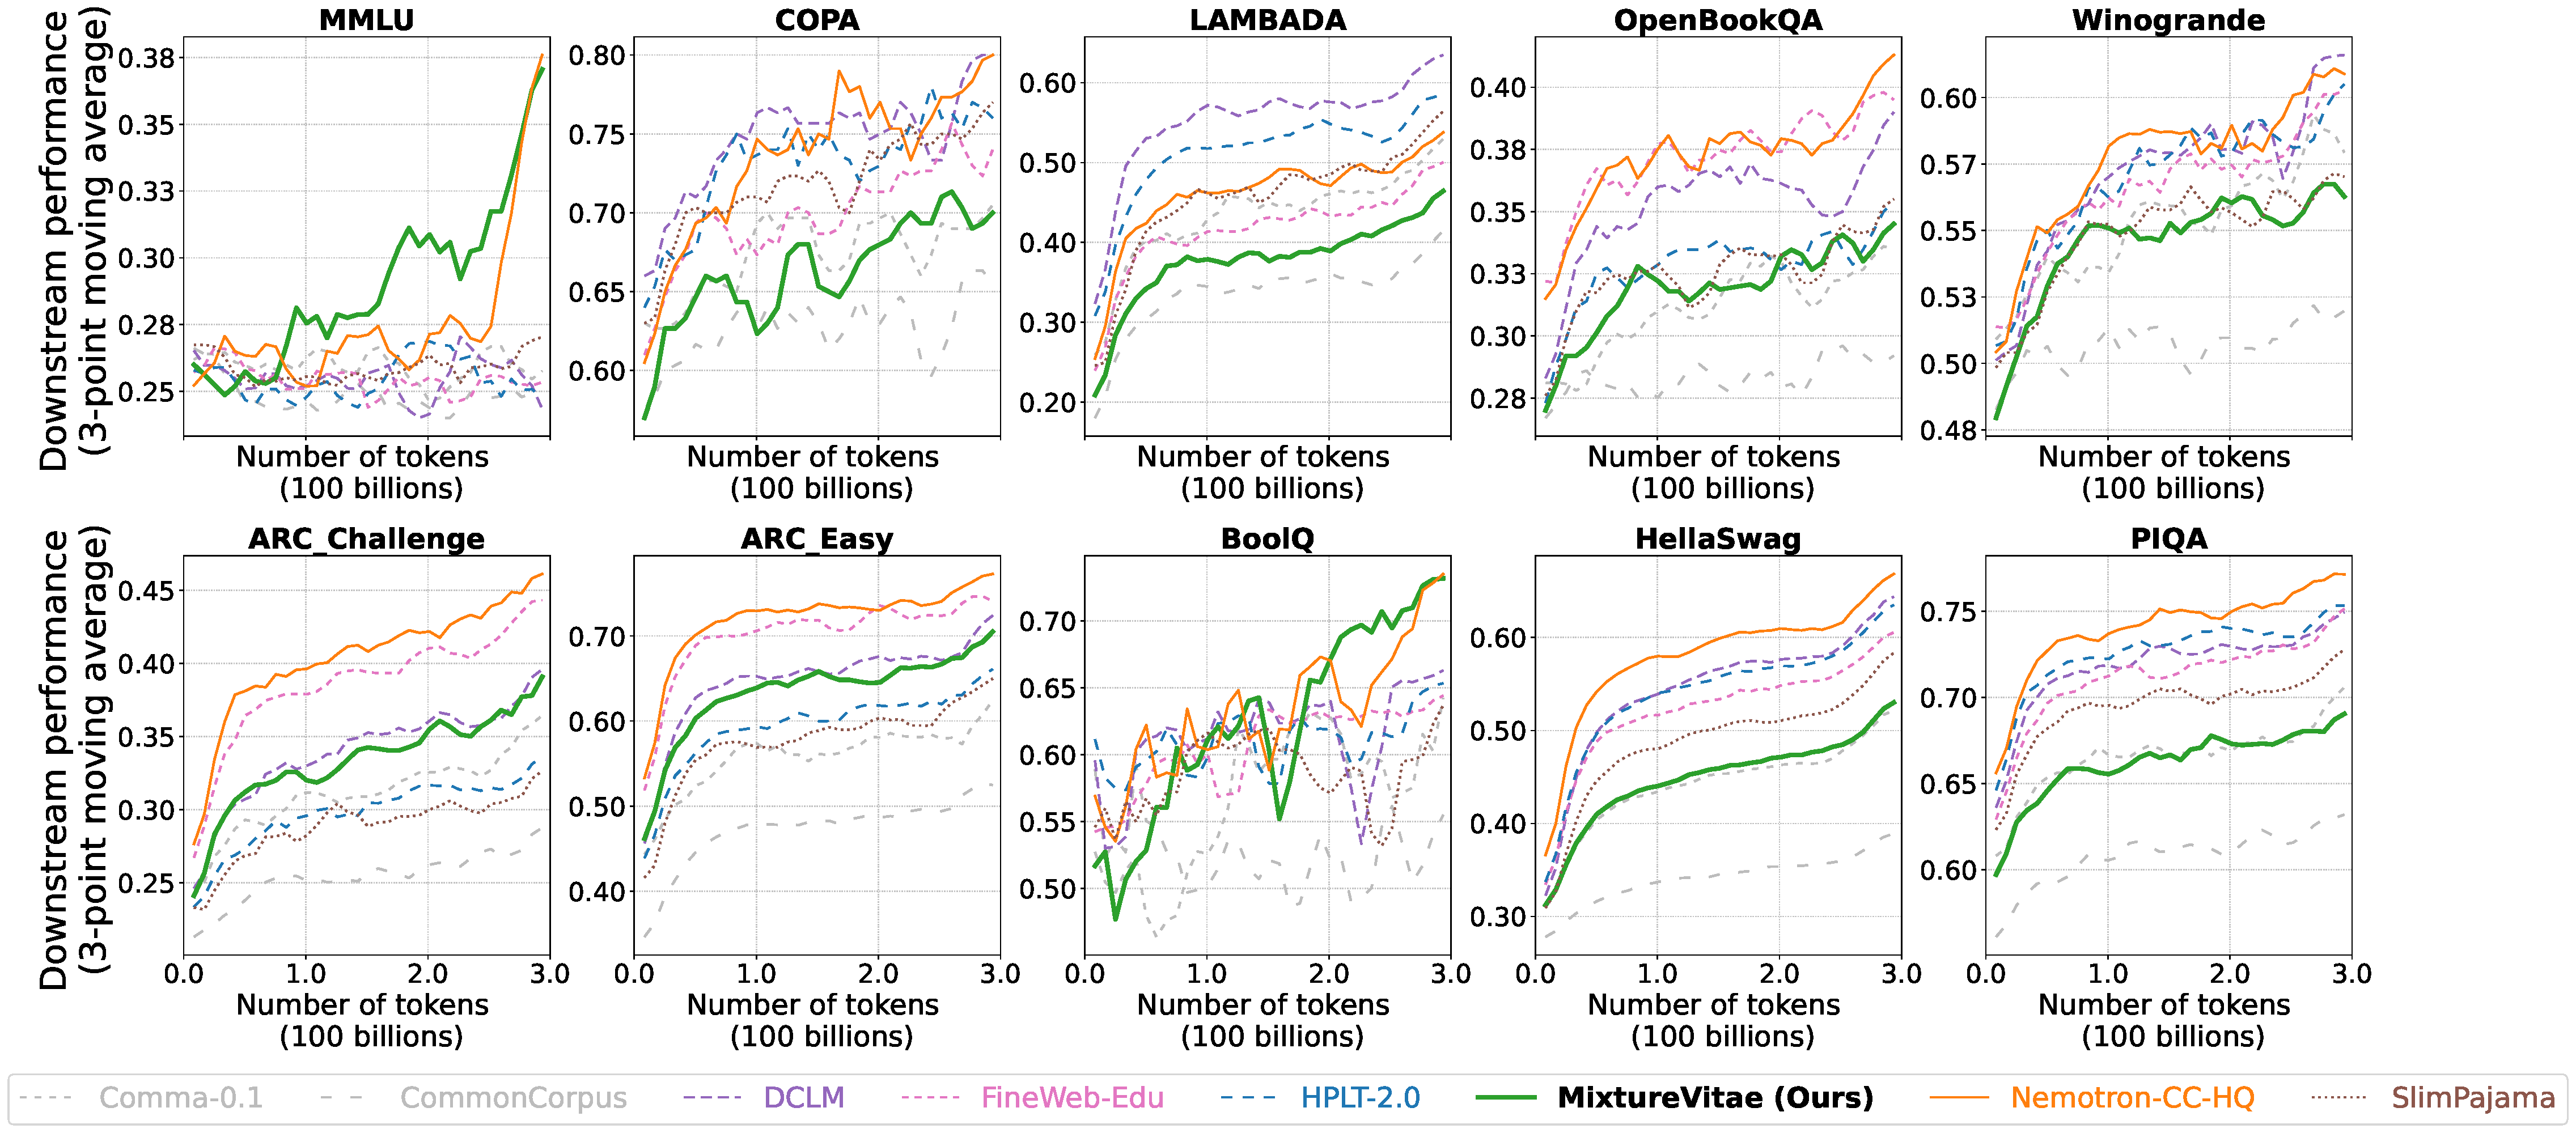
\includegraphics[width=1\linewidth]{figures/per_dataset_perf.pdf}
    \caption{Comparing performance of 1.7B model trained on \MixtureVitae{} and baseline datasets for a 300B token budget. While some evaluations provide clear dataset rankings (e.g. ARC, Hellaswag, Lambada), others do not provide a good signal for dataset comparison, on an individual basis.}
    \label{fig:per_dataset_performance}
\end{figure}
% --- figure with task groups - DISCARDED 
% \begin{figure}[htb!]
%     \centering
%         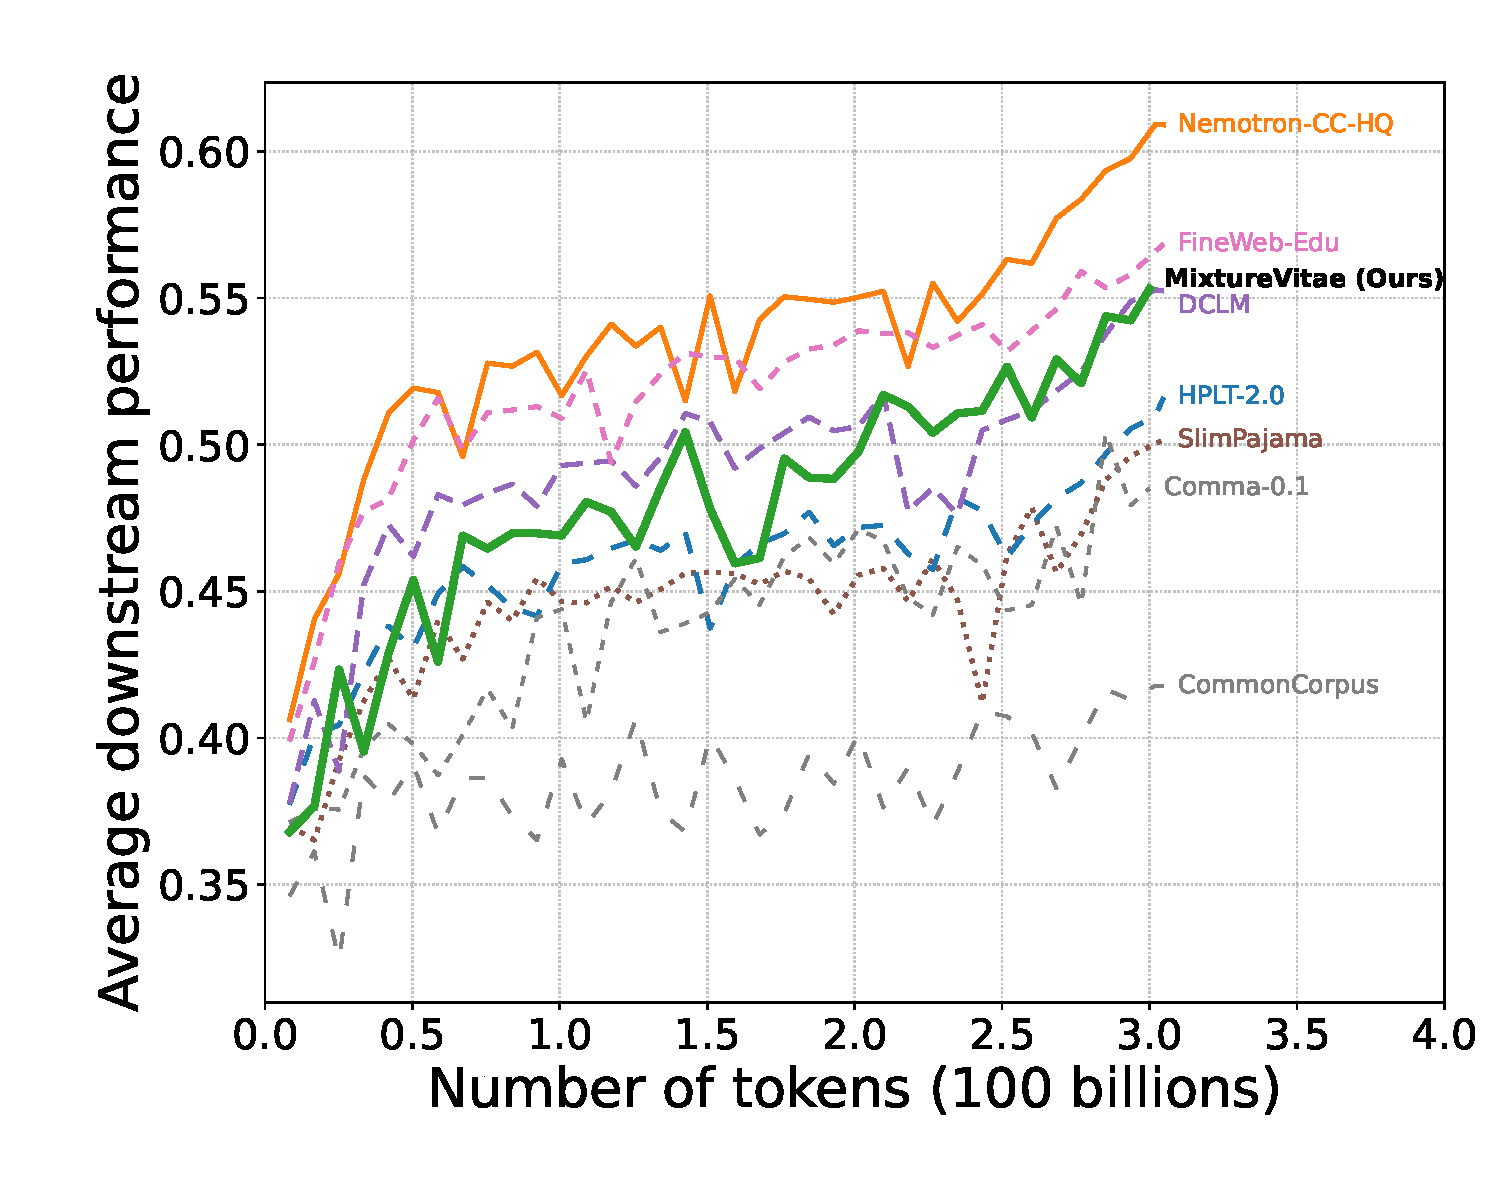
\includegraphics[width=\linewidth]{figures/300B_results_qa_plot_clustered_avg.pdf}
%         \vspace*{-0.5cm}
%           \caption{Average performance on Question Answering tasks (ARC-Challenge, ARC-Easy, BoolQ, OpenBookQA).}
%         \label{fig:average_qna_performance}
%     \end{subfigure}%
%     \hfill % Add horizontal spacing
%     \begin{subfigure}[t]{0.49\textwidth}
%         \centering
%         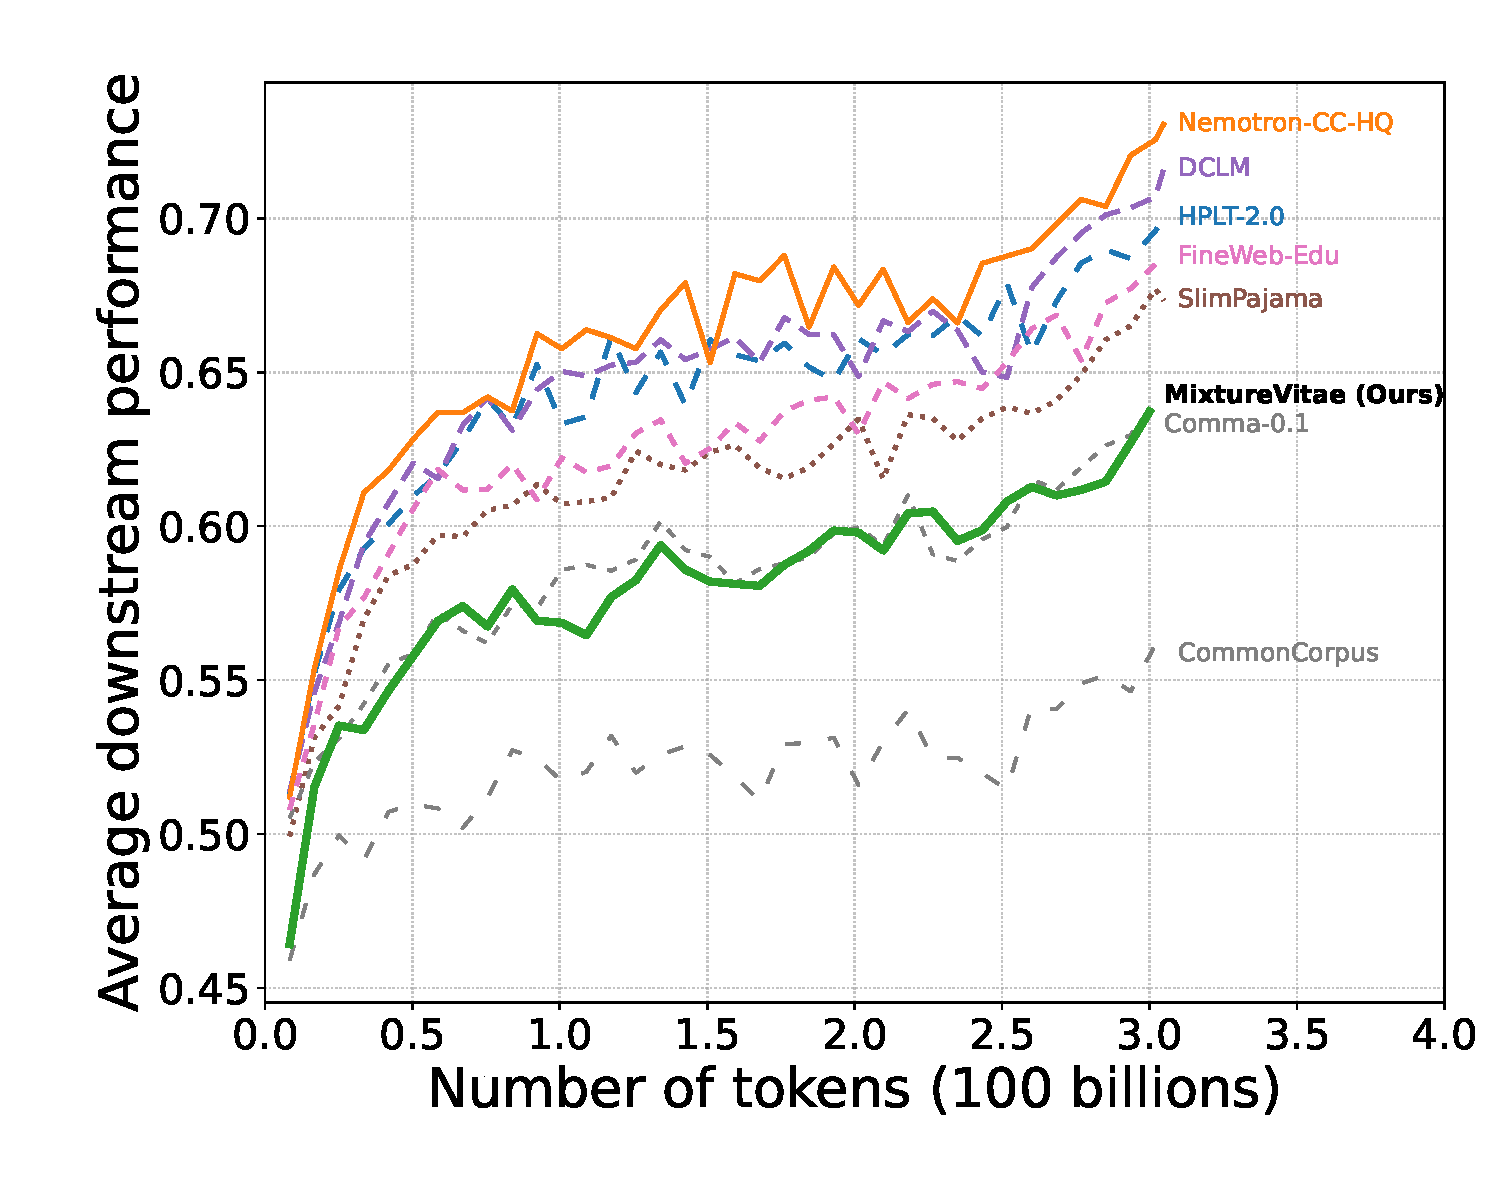
\includegraphics[width=\linewidth]{figures/300B_results_common_sense_plot_clustered_avg.pdf}
%         \vspace*{-0.5cm}
%          \caption{Average performance on Common Sense Knowledge tasks (COPA, HellaSwag, PIQA, Winogrande).}
%         \label{fig:average_common_sense_performance}
%     \end{subfigure}

%     \caption{Performance comparison of pretraining datasets for a 1.7B-parameter model trained up to a 300B token budget, showing downstream accuracy as a function of the number of training tokens.

\subsection{Performance at 50B Tokens Scale.} 

\begin{figure}[htbp]
    \centering
    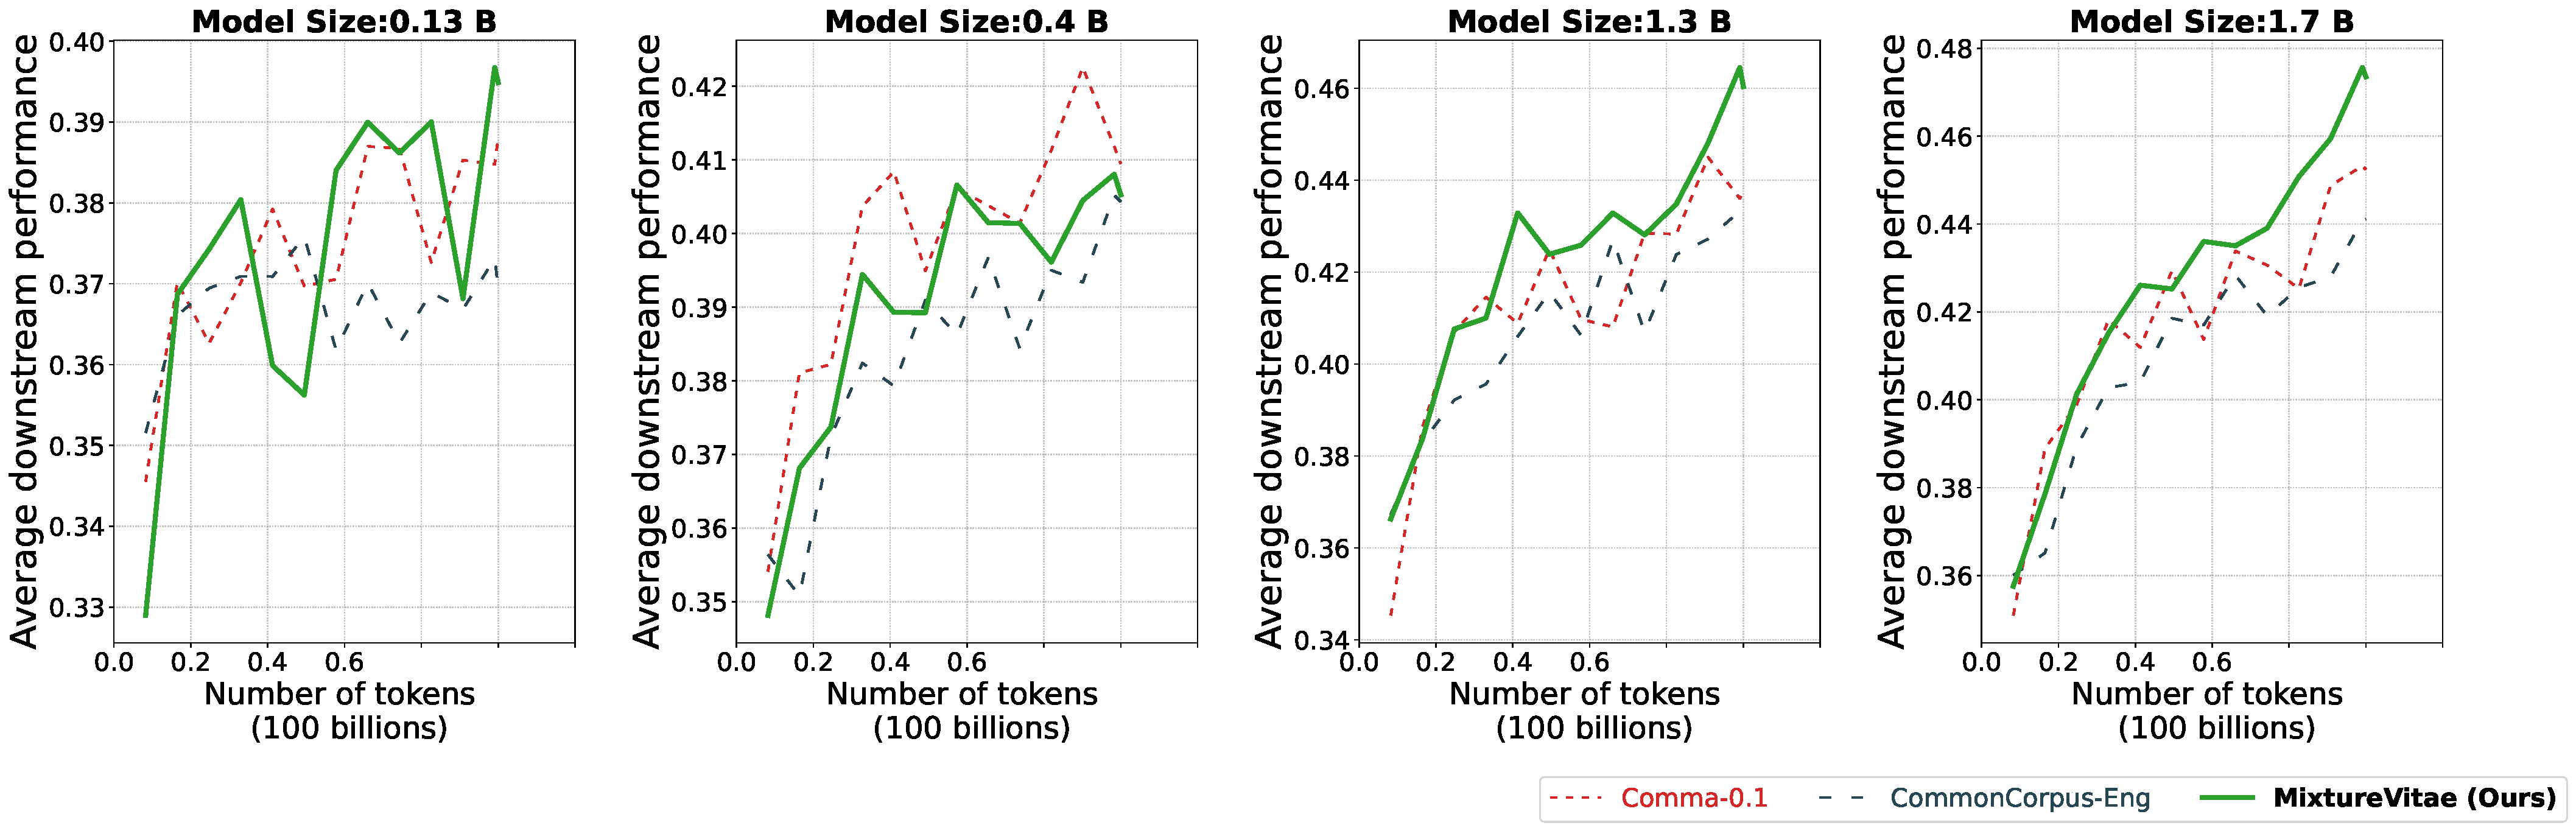
\includegraphics[width=\linewidth]{figures/50B_perf.pdf}
    \caption{Average performance of permissive datasets after 50B training tokens. \MixtureVitae{} shows an early and consistent lead at larger model scales.}
    \label{fig:50b_avg_perf}
\end{figure}

\begin{figure}[htbp]
    \centering
    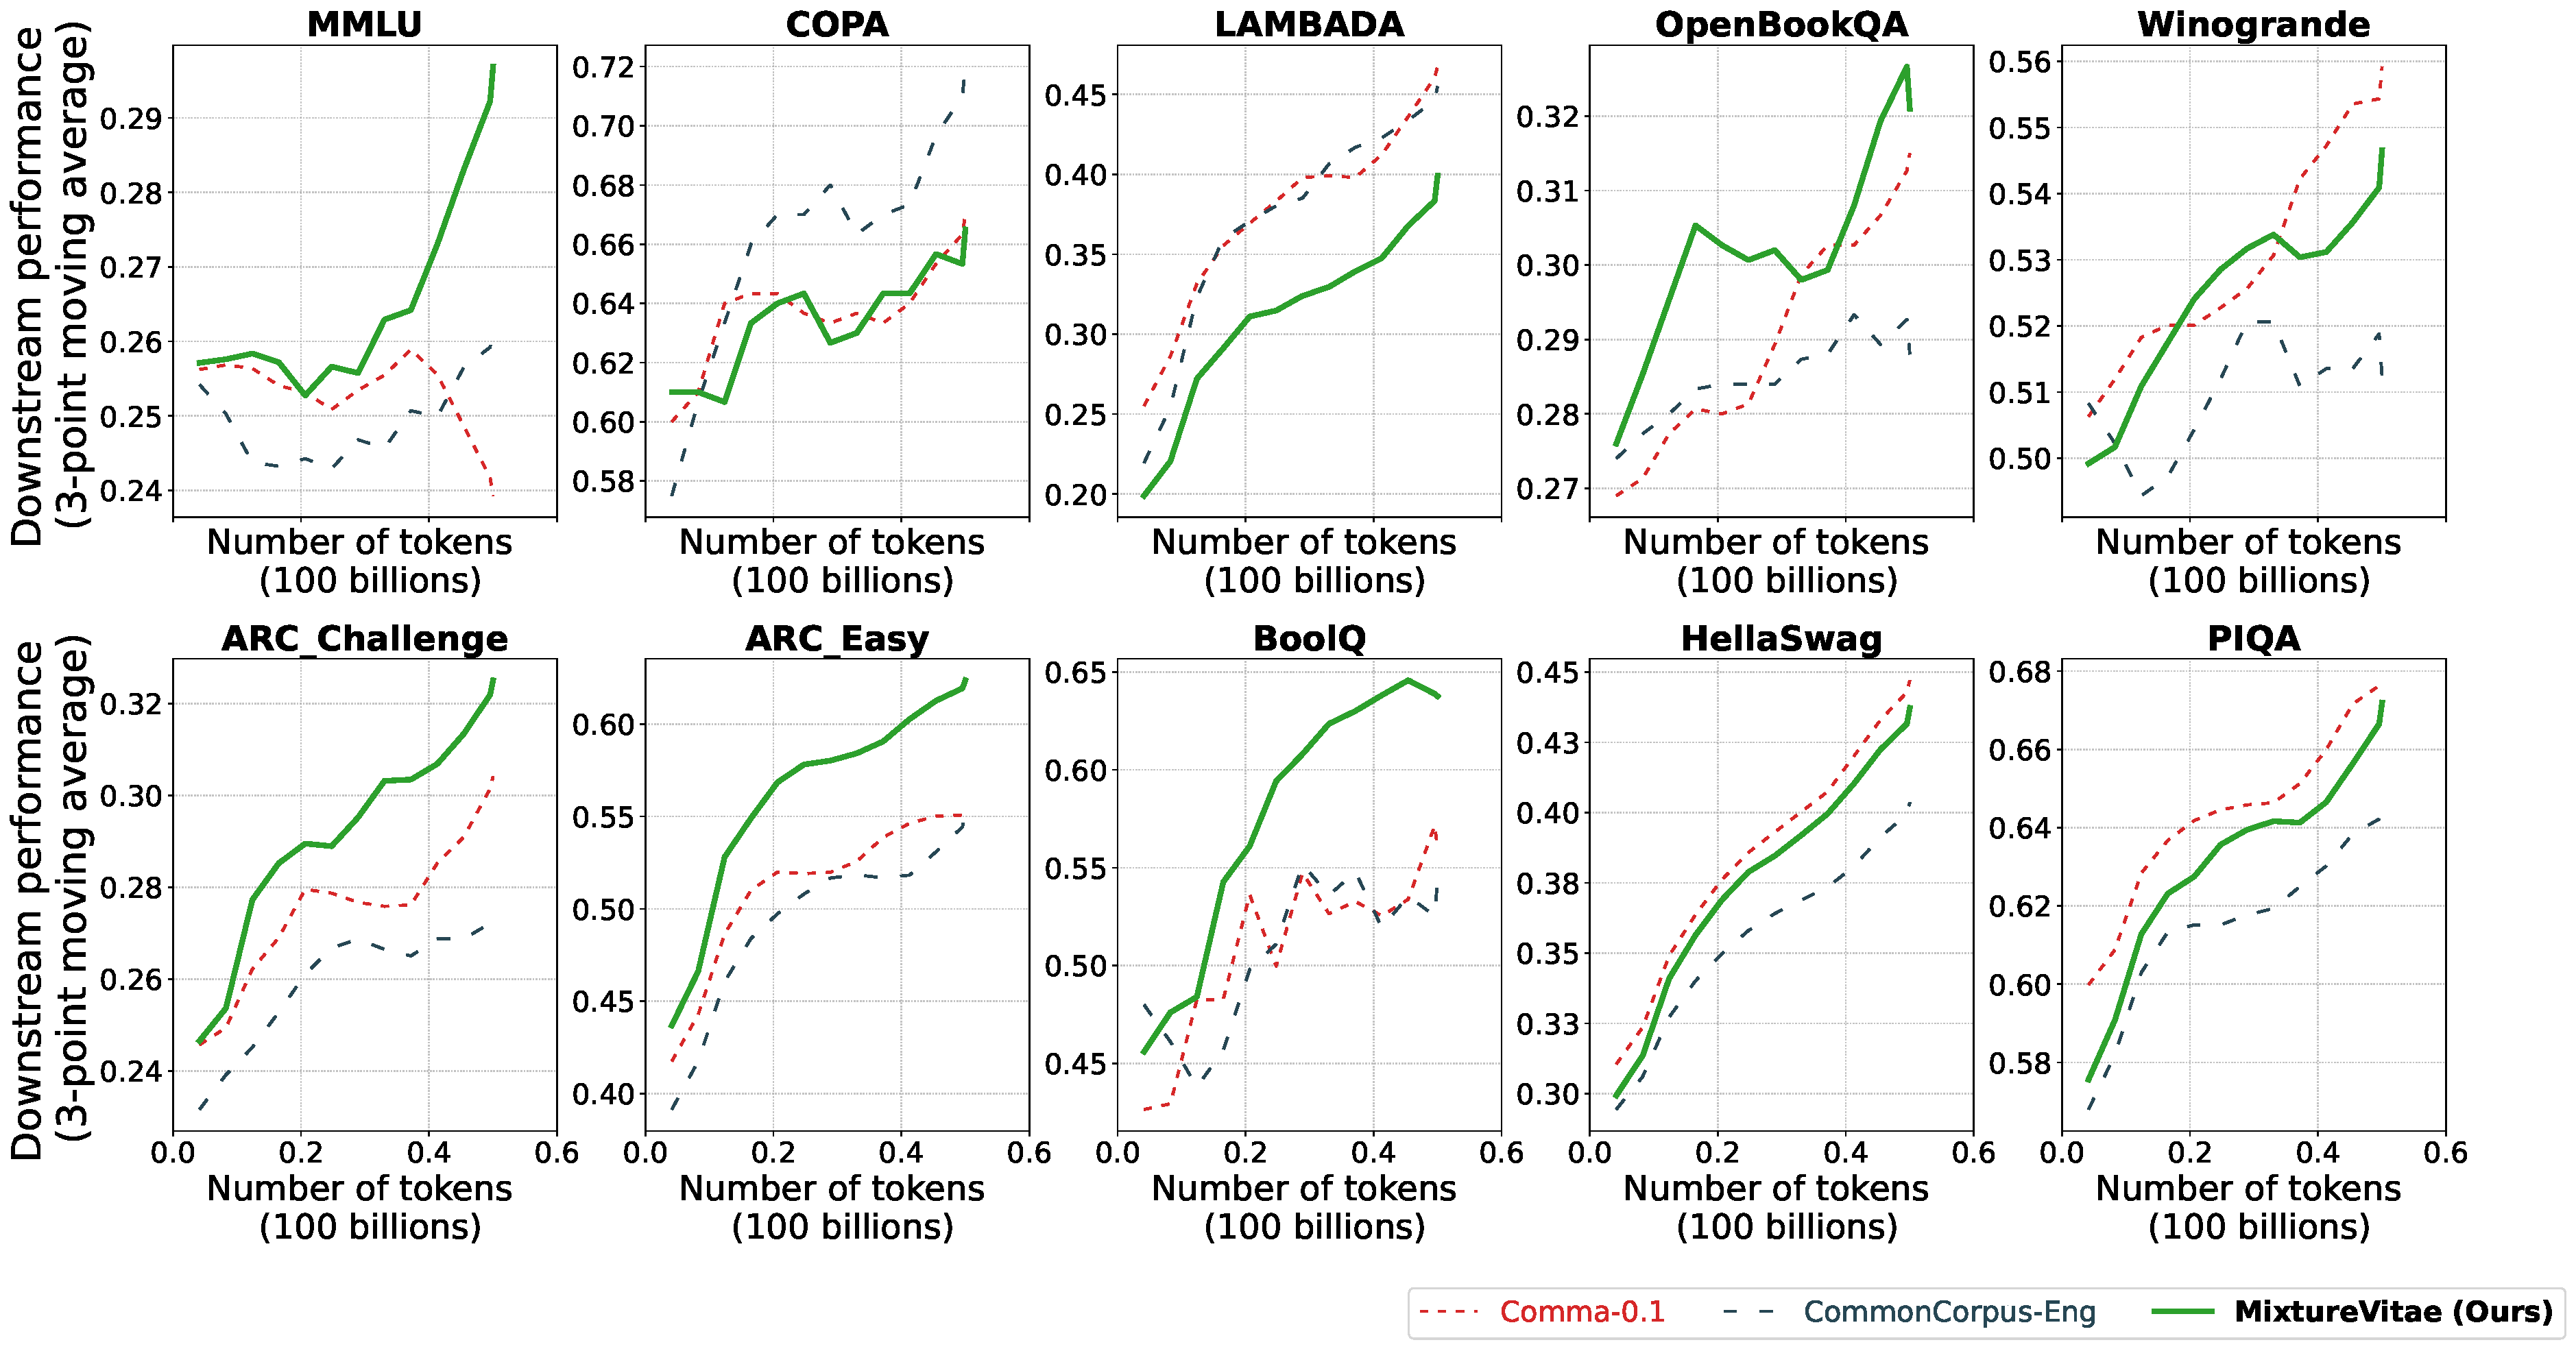
\includegraphics[width=\linewidth]{figures/50B_perf_per_dataset.pdf}
    \caption{Per-benchmark performance of permissive datasets after 50B training tokens. \MixtureVitae{}'s advantage on MMLU is apparent even at this early stage.}
    \label{fig:50b_per_benchmark_perf}
\end{figure}

\label{app:50b_exp} To assess performance on a smaller reference tokens scale, we also evaluated models trained on a 50B token subset of each  dataset. The results, shown in Figure~\ref{fig:50b_avg_perf} and Figure~\ref{fig:50b_per_benchmark_perf}, indicate that the advantages of \MixtureVitae{} manifest already at the smaller token scales. Figure~\ref{fig:50b_avg_perf} shows that \MixtureVitae{} establishes a consistent performance lead over other permissive datasets within the first 50B tokens, especially at the 1.3B and 1.7B model scales. The per-benchmark analysis further reinforces this finding (see Figure~\ref{fig:50b_per_benchmark_perf}). On MMLU, \MixtureVitae{} is the only permissive dataset to show a significant learning signal early in training, demonstrating that its composition provides immediate benefits, which might be both due to knowledge rich and instruction like content. Arguably, this suggests that the reasoning capability shown by \MixtureVitae{} is not a late-stage phenomenon but rather an indication of efficient instillation from the early stages of training. This strong initial performance underscores the learning efficiency of \MixtureVitae{}, making it a compelling choice for achieving high performance with less computational cost.


\subsection{Model Red Teaming}
\label{app:red_teaming}
To evaluate the safety of the model trained on \MixtureVitae{} for 300B tokens, we performed a red-teaming analysis to measure the Attack Success Rate (ASR) against three standard benchmarks: \textbf{ToxiGen} \citep{hartvigsen2022toxigen}, \textbf{Do-Not-Answer} \citep{wang2024not}, and \textbf{AdvBench} \citep{zou2023universal}. The results (Table~\ref{tab:model_performance}) shows that our model is competitive with the baselines.

The model responses were evaluated using two safety classifiers: (i) \textbf{Llama Guard-8B} \citep{inan2023llamaguardllmbasedinputoutput}, used to evaluate the \textbf{Do-Not-Answer} and \textbf{AdvBench} datasets, while (ii) the \textbf{toxigen\_roberta} classifier \citep{logacheva-etal-2022-paradetox} was used for the \textbf{ToxiGen} benchmark.

\begin{table}[ht]
\centering
% \resizebox{0.8\textwidth}{!}
% \small
\caption{Attack Success Rate in \%, lower is better. All models are trained with the same \textbf{open-sci-ref} procedure (300B-token budget) while varying only the pretraining dataset.}
\label{tab:model_performance}
\begin{tabular}{lcccc}
\toprule
\textbf{Benchmark} & \textbf{\MixtureVitae} & \textbf{Comma} & \textbf{CommonCorpus-Eng} & \textbf{Nemotron-HQ-CC} \\
\midrule
ToxiGen & 8.07 & 9.04 & 12.77 & 10.21 \\
Do-Not-Answer & 28.22 & 24.71 & 21.62 & 20.98 \\
AdvBench & 86.92 & 92.12 & 70.58 & 85.77 \\
\bottomrule
\end{tabular}
\end{table}


% \subsection{Results on Math and Coding}

% \begin{table}
% \small
% \center
% \begin{tabular}{lrrrr}
\toprule
 & GSM8K  & HumanEval & MBPP & Average \\
\midrule
\MixtureVitae{} & \textbf{0.53} & \textbf{0.30} & \textbf{0.38} & \textbf{0.40} \\
Comma-0.1 & 0.06 & 0.13 & 0.21 & 0.13 \\
CommonCorpus & 0.02 & 0.05 & 0.00 & 0.02 \\
\midrule
SlimPajama & 0.02 & 0.05 & 0.00 & 0.03 \\
Nemotron-CC-HQ & 0.03 & 0.02 & 0.00 & 0.02 \\
DCLM & 0.02 & 0.01 & 0.00 & 0.01 \\
HPLT-2.0 & 0.02 & 0.00 & 0.00 & 0.01 \\
FineWeb & 0.03 & 0.00 & 0.00 & 0.01 \\
C4 & 0.03 & 0.00 & 0.00 & 0.01 \\
\bottomrule
\end{tabular}
% \caption{Results on Math and Coding tasks. Datasets are shown by group including permissive ones (top) and others (bottom). \label{tab:mathcoding}}
% \end{table}

% In Table \ref{tab:mathcoding}, we show the performance of several models trained on 300B tokens on multiple datasets for GSM8K \cite{cobbe2021training}, HumanEval \cite{austin2021program} and MBPP \cite{chen2021evaluating} where we report exact-match for GSM8K and pass@1 for HumanEval and MBPP.

% % \begin{table}[ht]
% % \centering
% % \begin{tabular}{lrrrrrr}
% % \toprule
% % Model & GPQA-D & GPQA & MATH & IF-Eval & GSM8K & Average \\
% % \midrule
% % MixtureVitae, 300BT & 0.303 & 0.241 & 0.110 & 0.207 & 0.500 & 0.272 \\
% % SmolLM2 & 0.197 & 0.252 & 0.094 & 0.174 & 0.287 & 0.201 \\
% % Nemotron-HQ 1T & 0.298 & 0.254 & 0.033 & 0.135 & 0.047 & 0.154 \\
% % DCLM, 300B & 0.323 & 0.221 & 0.026 & 0.126 & 0.026 & 0.144 \\
% % Nemotron-HQ, 300B & 0.167 & 0.158 & 0.031 & 0.091 & 0.031 & 0.096 \\
% % \bottomrule
% % \end{tabular}
% % \caption{All 1.7b models}
% % \end{table}


% % \begin{table}[ht]
% % \centering
% % \caption{Unified 1.7B Model Results (Ablation and Baseline)}
% % \label{tab:unified-models-final}
% % \begin{tabular}{llcrrrrrr}
% % \toprule
% % Model & Training Dataset & \shortstack{Training \\ Tokens} & GPQA-D & GPQA & IF-Eval & GSM8K & HumanEval & MBPP \\
% % \midrule
% % \multirow{10}{*}{\textbf{open-sci-ref}} & \textbf{MixtureVitae} & \textbf{300B} & \textbf{0.303} & \textbf{0.241} & \textbf{0.207} & \textbf{0.500} & \textbf{0.53} & \textbf{0.30} \\
% %  & Nemotron-HQ & 1T & 0.298 & 0.254 & 0.135 & 0.047 & --- & --- \\
% %  & DCLM & 300B & 0.323 & 0.221 & 0.026 & 0.126 & 0.02 & 0.00 \\
% %  & Nemotron-HQ & 300B & 0.167 & 0.158 & 0.031 & 0.091 & 0.03 & 0.00 \\
% %  & Comma & 300B & --- & --- & --- & 0.06 & 0.13 & 0.21 \\
% %  & CommonCorpus & 300B & --- & --- & --- & 0.02 & 0.05 & 0.00 \\
% %  & SlimPajama & 300B & --- & --- & --- & 0.02 & 0.05 & 0.00 \\
% %  & HPLT-2.0 & 300B & --- & --- & --- & 0.02 & 0.01 & 0.00 \\
% %  & FineWeb & 300B & 300B & --- & --- & --- & 0.03 & 0.00 \\
% %  & C4 & 300B & --- & --- & --- & 0.03 & 0.00 & 0.00 \\
% % \midrule
% % \textbf{SmolLM2} & \textbf{\textit{Baseline Model}} & \textbf{11T} & \textbf{0.197} & \textbf{0.252} & \textbf{0.174} & \textbf{0.287} & \textbf{---} & \textbf{---} \\
% % \bottomrule
% % \end{tabular}
% % \end{table}
% \begin{table}[ht]
% \scriptsize
% \centering
% \caption{Evaluation results on reasoning tasks for 1.7B models. For evaluation setting refer to table \ref{tab:eval-settings}}
% \begin{tabular}{llrrrrrr}
% \toprule
% Training Dataset & \#Tokens & GPQA-D & GPQA & MATH & IFEval & GSM8K & Avg. \\
% \midrule
% \textbf{MixtureVitae (ours)} & 300B & 0.27 & 0.24 & \textbf{0.11} & 0.19 & \textbf{0.51} & \textbf{0.26} \\
% \midrule
% SmolLM2-1.7B \cite{allal2025smollm2} & 11T & 0.23 & \textbf{0.27} & 0.09 & 0.18 & 0.29 & 0.21 \\
% Nemotron-CC-HQ \cite{su2025nemotroncctransformingcommoncrawl} & 1T & 0.29 & 0.26 & 0.03 & 0.13 & 0.05 & 0.15 \\
% DCLM \cite{li2024datacomplm} & 300B & \textbf{0.32} & 0.22 & 0.03 & 0.13 & 0.03 & 0.14 \\
% SlimPajama \cite{shen2024slimpajamadcunderstandingdatacombinations} & 300B & 0.25 & 0.26 & 0.02 & 0.14 & 0.02 & 0.14 \\
% DCLM \cite{li2024datacomplm} & 1T & 0.24 & 0.24 & 0.03 & 0.15 & 0.03 & 0.14 \\
% HPLT-2.0 \cite{hplt2024} & 300B & 0.20 & 0.24 & 0.01 & 0.17 & 0.02 & 0.13 \\
% CommonCorpus \cite{commoncorpus2023} & 300B & 0.19 & 0.19 & 0.02 & 0.13 & 0.02 & 0.11 \\
% C4 \cite{raffel2020exploring} & 300B & 0.15 & 0.13 & 0.00 & \textbf{0.20} & 0.02 & 0.10 \\
% Nemotron-CC-HQ \cite{su2025nemotroncctransformingcommoncrawl} & 300B & 0.17 & 0.16 & 0.03 & 0.09 & 0.03 & 0.10 \\
% \bottomrule
% \end{tabular}
% \label{tab:extra-evals}
% \end{table}

% \begin{table}[ht]
% \centering
% \scriptsize
% \caption{Evaluation settings for reasoning tasks. For evaluation we used LM Evaluation Harness\cite{eval-harness}.}
% \begin{tabular}{lccl}
% \hline
% Task & Short Name & \# of Shots & Metrics \\
% \hline
% MATH \cite{hendrycksmath2021} & MATH & 4 & exact\_match \\
% GSM8k CoT \cite{cobbe2021training} & GSM8K & 4 & exact\_match, flexible-extract \\
% GPQA CoT \cite{rein2023gpqa} & GPQA & 4 & exact\_match, flexible-extract \\
% IFEval \cite{zhou2023instructionfollowing} & IFEval & -- & prompt\_level\_strict\_acc \\
% GPQA Diamond CoT \cite{rein2023gpqa} & GPQA-D & 4 & exact\_match, flexible-extract \\
% \hline
% \end{tabular}
% \label{tab:eval-settings}
% \end{table}

% \begin{table}[ht]
% \centering
% \scriptsize
% \label{tab:eval_ablations_math_code}
% \caption{Evaluation of ablation models on reasoning benchmarks.}
% \begin{tabular}{llrrrrrrrr}
% \toprule
% Training Dataset & Tokens & GPQA-D & GPQA & MATH & IF-Eval & GSM8K & HumanEval & MBPP & avg \\
% \midrule
% MixtureVitae & 300B & 0.27 & 0.24 & 0.11 & 0.19 & 0.51 & 0.31 & 0.38 & 0.29 \\
% MixtureVitae-300BT-instruct & 80B & 0.22 & 0.24 & 0.07 & 0.17 & 0.57 & 0.42 & 0.24 & 0.28 \\
% MixtureVitae-300BT-web\_instruct & 100B & 0.21 & 0.21 & 0.11 & 0.17 & 0.53 & 0.37 & 0.31 & 0.27 \\
% MixtureVitae-300BT & 80B & 0.24 & 0.24 & 0.07 & 0.14 & 0.49 & 0.30 & 0.29 & 0.25 \\
% MixtureVitae-300BT-curated\_instruct & 100B & 0.21 & 0.24 & 0.09 & 0.18 & 0.41 & 0.30 & 0.33 & 0.25 \\
% MixtureVitae-300BT & 100B & 0.21 & 0.21 & 0.09 & 0.14 & 0.47 & 0.27 & 0.34 & 0.25 \\
% SmolLM2-1.7B & 11T & 0.23 & 0.27 & 0.09 & 0.18 & 0.29 & 0.01 & 0.35 & 0.20 \\
% Comma0.1 & 300BT & 0.25 & 0.23 & 0.03 & 0.19 & 0.10 & 0.13 & 0.22 & 0.16 \\
% MixtureVitae-300BT-curated & 80B & 0.22 & 0.26 & 0.03 & 0.20 & 0.03 & 0.12 & 0.13 & 0.14 \\
% MixtureVitae-300BT-web\_curated & 100B & 0.24 & 0.23 & 0.03 & 0.19 & 0.03 & 0.10 & 0.14 & 0.14 \\
% \bottomrule
% \end{tabular}
% \end{table}


% \begin{table}[h!]
% \centering
% \scriptsize
% \begin{tabular}{lcc}
% \hline
% Dataset & Number of samples & Accuracy \\
% \hline
% HumanEval & 164 & 0.30 \\
% HumanEval decontaminated & 75 & 0.23 \\
% MBPP       & 500 & 0.38 \\
% MBPP decontaminated & 331 & 0.38 \\
% \hline
% \end{tabular}
% \end{table}
